
Neste capítulo será apresentado em detalhes os resultados obtidos para o classificador base e o classificador proposto.

\section{\textit{Classificador Base Resultados Iniciais}}\label{sec:Cap4_ResultadosPreliminares}


O classificador base pôde ser mensurado pelas métricas $F_2$ e áreas das curvas ROC e PR. A partir da matriz confusão podemos obter com granularidade o comportamento do classificador. Também é possível notar experimentalmente o fato da acurácia em classes raras não refletir a qualidade do modelo: mesmo classificando apenas um verdadeiro positivo corretamente, obteve acurácia de 99,46\% para a classe Queimada, observando sua matriz confusão.

\begin{figure}[!ht]
    \centering
    \includegraphics[width=0.8\columnwidth]{Imagens/results/rsp-resnet-50_planet_pt/Matrizes confusão.jpg}
    \caption{ Matriz Confusão Resnet-50
    Fonte: Autor}
    \label{fig:Matriz Confusao Resnet50}
\end{figure} 


O desempenho do modelo base para cada classe foi sumarizado a seguir, em ordem crescente de métrica $F_2$. O desempenho do modelo para as diferentes classes foi muito discrepante, expressivamente abaixo para as classes mais raras. O classificador atinge resultados satisfatórios para classes mais abundantes, como o esperado. Contudo, o que os modelos podem se distinguir são nas classes raras. Para isso serão comparados os resultados globais e das classes raras, definidas como possuindo menos de 5\% do total de amostras, expostas na tabela \ref{table:Classes raras}. Dessa forma é possível de comparar a capacidade de generalização dos modelos e do viés indutivo.

\begin{table}[h!]
    \caption{Resultados do Modelo ResNet50}
    \centering
\begin{tabular}{*{6}{c}}
    \toprule
    {} &              Rótulo &  F2    &  Limiar   &  PR AUC &  AUC Ingênuo \\
    \midrule
    15 &         slash burn &  0,030 &      0,230 &   0,145 &       0,005 \\
    3  &           blooming &  0,140 &      0,130 &   0,096 &       0,008 \\
    4  &          blow down &  0,268 &      0,190 &   0,245 &       0,003 \\
    2  &        bare ground &  0,373 &      0,210 &   0,316 &       0,024 \\
    14 &  selective logging &  0,422 &      0,090 &   0,401 &       0,010 \\
    7  &  conventional mine &  0,579 &      0,170 &   0,536 &       0,002 \\
    8  &        cultivation &  0,674 &      0,130 &   0,650 &       0,114 \\
    9  &         habitation &  0,769 &      0,130 &   0,802 &       0,093 \\
    10 &               haze &  0,774 &      0,210 &   0,784 &       0,063 \\
    16 &              water &  0,836 &      0,210 &   0,892 &       0,181 \\
    1  &     artisinal mine &  0,840 &      0,190 &   0,880 &       0,008 \\
    13 &               road &  0,864 &      0,210 &   0,916 &       0,200 \\
    0  &        agriculture &  0,890 &      0,250 &   0,929 &       0,306 \\
    6  &             cloudy &  0,910 &      0,230 &   0,946 &       0,051 \\
    11 &      partly cloudy &  0,938 &      0,210 &   0,972 &       0,173 \\
    5  &              clear &  0,978 &      0,210 &   0,996 &       0,713 \\
    12 &            primary &  0,992 &      0,190 &   0,999 &       0,928 \\
    17 &             global &  0,928 &      0,188 &   0,677 &       0,170 \\
    \bottomrule
\end{tabular}
\label{table:ResultadosResnet50}
\end{table}

\begin{table}[h!]
    \caption{Classes Raras Dataset \textit{Planet} — Valores do conjunto de dados inteiro}
    \centering
\begin{tabular}{*{4}{c}}
    \toprule
    Classe                  &            Rótulo &  Amostras      &  Proporção (\%) \\
    \midrule
    Mina Convencional       & conventional mine &        100     &       0,247 \\
    Roça de Ventos          &         blow down &        101     &       0,250 \\
    Queimada                &        slash burn &        209     &       0,516 \\
    Florescimento           &          blooming &        332     &       0,820 \\
    Garimpo                 &    artisinal mine &        339     &       0,837 \\
    Desmatamento Seletivo   & selective logging &        340     &       0,840 \\
    Área Descoberta         &       bare ground &        862     &       2,129 \\
    Todo conjunto de dados  &            global &        40479   &       100.0 \\
    \bottomrule
\end{tabular}
\label{table:Classes raras}
\end{table}

\begin{figure}[!ht]
    \centering
    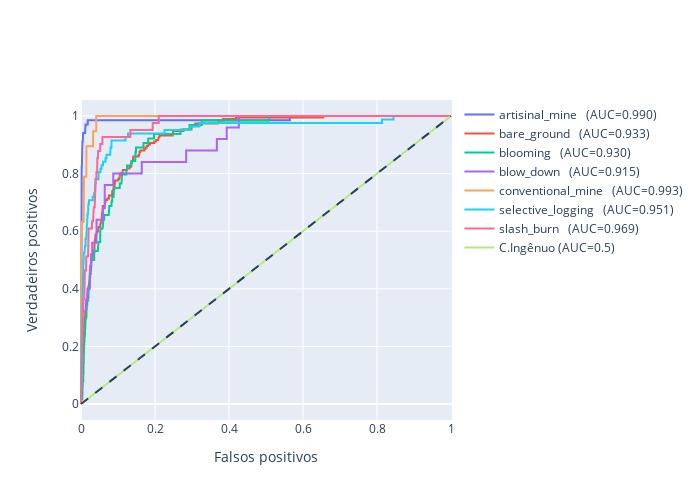
\includegraphics[width=0.8\columnwidth]{Imagens/results/rsp-resnet-50_planet_pt/Curva COR para classes raras.jpg}
    \caption{ Curva COR para o modelo base. Fonte: Autor}
   \label{fig:CurvaCORResnet50}
\end{figure} 

Temos ainda que a métrica AUC-ROC apresentou-se pouco capaz de distinguir a atuação do modelo, como demonstra a figura \ref{fig:CurvaCORResnet50}: Classes com baixos escores tiveram áreas similares de classes performáticas. Portanto, a análise a seguir se delimitará às classes raras e com escores precisão-revocação.

\section{\textit{Classificador Base Análise Para classes Escassas}}\label{sec:Cap4_ClassifiadorBase}

Sintetizando os mesmos resultados anteriores para as classes escassas da tabela \ref{table:Classes raras}, temos a tabela \ref{table:ResultadosResnet50ClassesRaras}. Com exceção da classe de Garimpo, o modelo teve baixa desempenho, em relação as demais classes removidas. Podemos constatar o mesmo observando a curva PR, da figura \ref{fig:CurvaPRResnet50}. Tais classes também obtiveram a curva característica de um classificador pobre. 



\begin{table}[h!]
    \caption{Resultados do Modelo Base}
    \centering
\begin{tabular}{*{6}{c}}
    \toprule
    \midrule
                 Rótulo &  F2    & PR AUC &  AUC Ingênuo \\
             slash burn &  0,030 &  0,145 &       0,005 \\
               blooming &  0,140 &  0,096 &       0,008 \\
              blow down &  0,268 &  0,245 &       0,003 \\
            bare ground &  0,373 &  0,316 &       0,024 \\
      selective logging &  0,422 &  0,401 &       0,010 \\
      conventional mine &  0,579 &  0,536 &       0,002 \\
         artisinal mine &  0,840 &  0,880 &       0,008 \\
                 global &  0,928 &  0,677 &       0,170 \\         
    \bottomrule
\end{tabular}
\label{table:ResultadosResnet50ClassesRaras}
\end{table}
  

\begin{figure}[!ht]
    \centering
    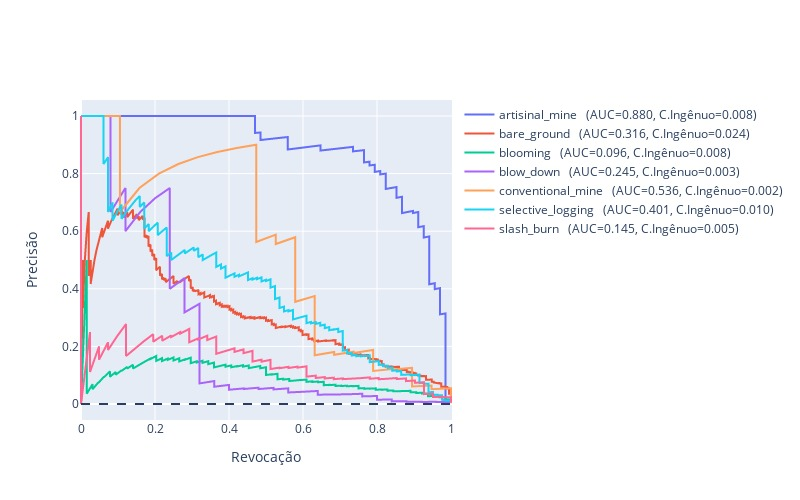
\includegraphics[width=\columnwidth]{Imagens/results/rsp-resnet-50_planet_pt/Curva PR para classes raras.jpg}
    \caption{ Curva PR para o modelo base.
    Fonte: Autor}
   \label{fig:CurvaPRResnet50}
\end{figure}   

   


\section{\textit{Classificador Proposto}}\label{sec:Cap4_ClassifiadorProposto}

Reproduzindo os mesmos procedimentos anteriores para o modelo Swin-T os mesmos resultados anteriores para as classes escassas da tabela \ref{table:Classes raras}, temos a tabela \ref{table:ResultadosSwinT}. 

\begin{figure}[!ht]
    \centering
    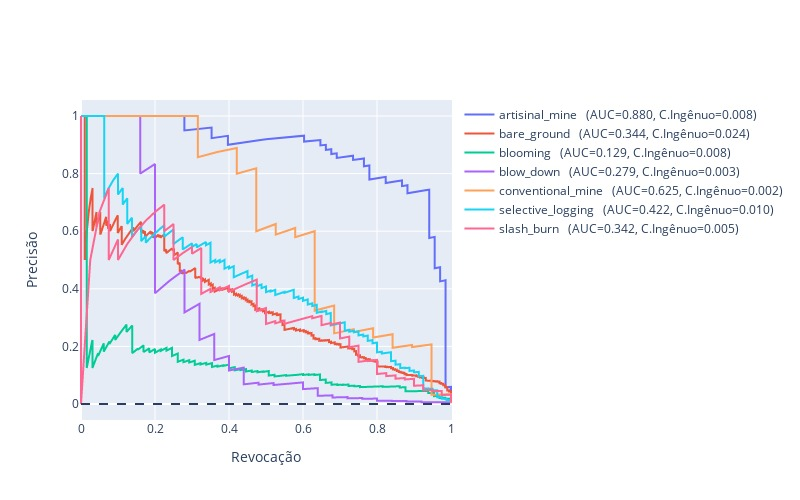
\includegraphics[width=\columnwidth]{Imagens/results/rsp-swin-t_planet_pt/Curva PR para classes raras.jpg}
    \caption{ Arquitetura de modelo Swin-T proposto.
    Fonte: Autor}
    \label{fig:CurvaPRSwint}
\end{figure}   

\begin{table}[h!]
        \caption{Resultados do Modelo Swin-T}
        \centering
    \begin{tabular}{*{6}{c}}
        \toprule
                     Rótulo &  F2    &   PR AUC &  PR-AUC Class.Ingênuo \\
        \midrule
                  blooming &  0,230 &    0,129 &       0,008 \\
                slash burn &  0,338 &    0,342 &       0,005 \\
                 blow down &  0,310 &    0,279 &       0,003 \\
               bare ground &  0,447 &    0,344 &       0,024 \\
         selective logging &  0,475 &    0,422 &       0,010 \\
         conventional mine &  0,538 &    0,625 &       0,002 \\
            artisinal mine &  0,872 &    0,880 &       0,008 \\
                    global &  0,930 &    0,704 &       0,170 \\
        \bottomrule
    \end{tabular}
    \label{table:ResultadosSwinT}
\end{table}
    
    
\section{\textit{Comparação de resultados}}\label{sec:Cap4_Comparação de resultados}    

Nesta sessão compararemos a desempenho dos modelos. Podemos observar pela curva PR \ref{fig:CurvaPRSwint}que as classes mais desafiadoras permanecem distantes de um classificador ideal, contudo pode-se notar um aumento relevante nas métricas $F_2$, $PR_AUC$, portanto qualificando este classificador superior ao modelo base. Temos ainda que embora a métrica $F_2$ esteja distante de um classificador ideal, de valor próximo a 1, temos que ela ainda é bastante superior ao classificador ingênuo/aleatório. Comparando com trabalho de \cite{9701667}, de métrica $F_2$ de 0,878, concluímos que este classificador possui desempenho satisfatório.



\begin{table}[h!]
    \caption{ Comparação de resultados da métrica F2 entre Modelo base e proposto.}
    \centering
\begin{tabular}{*{6}{c}}
    \toprule
    Rótulo &F2-Resnet&F2-SwinT \\
    \midrule
            slash burn &  0,030 &  0,338 \\ 
              blooming &  0,140 &  0,230 \\
             blow down &  0,268 &  0,310 \\
           bare ground &  0,373 &  0,447 \\
     selective logging &  0,422 &  0,475 \\
     conventional mine &  0,579 &  0,538 \\
        artisinal mine &  0,840 &  0,872 \\
                global &  0,928 &  0,930 \\
    \bottomrule
\end{tabular}
\label{table:ResultadosSwinT-F2}
\end{table}



\begin{table}[h!]
    \caption{ Comparação de resultados da métrica PR-AUC entre Modelo base e proposto.}
    \centering
\begin{tabular}{*{6}{c}}
    \toprule
    Rótulo &PR-AUC-ResNet&PR-AUC-SwinT&PR-AUC Class.Ingênuo \\
    \midrule
            slash burn &       0,145 &      0,342 &     0,005 \\
              blooming &       0,096 &      0,129 &     0,008 \\
             blow down &       0,245 &      0,279 &     0,003 \\
           bare ground &       0,316 &      0,344 &     0,024 \\
     selective logging &       0,401 &      0,422 &     0,010 \\
     conventional mine &       0,536 &      0,625 &     0,002 \\
        artisinal mine &       0,880 &      0,880 &     0,008 \\
                global &       0,677 &      0,704 &     0,170 \\
    \bottomrule
\end{tabular}
\label{table:ResultadosSwinT-PR-AUC }
\end{table}

Através das tabelas \ref{table:ResultadosSwinT-PR-AUC } e \ref{table:ResultadosSwinT-F2}, podemos constatar que o modelo Swin apresentou melhor desempenho que o modelo base em todas as classes raras, bem como desempenho global, dado as métricas escolhidas. Dessa forma conseguiu melhor generalizar no contexto de poucas amostras.

Para uma validação final, podemos inspecionar visualmente as probabilidades marginais atribuídas a cada classe. É possível notar que para as classes raras, ainda são atribuídas probabilidades marginais inferiores, contudo também possuem menores limiares de classificação, como mostra a tabela de resultados e limiares presente nos anexos. \ref{table:AnexosResultadosSwinT}

\begin{figure}[!ht]
    \centering
    \includegraphics[width=\columnwidth]{Imagens/results/rsp-swin-t_planet_pt/Inferência para cada classe.jpg}
    \caption{ Arquitetura de modelo base.
    Fonte: Autor}
    \label{fig:InferenciaClassesSwin}
\end{figure}  